\newpage
\section{Implementacja}		%4

\subsection{Struktura kodu}
W projekcie, struktura kodu została zaprojektowana w sposób umożliwiający łatwą rozbudowę oraz utrzymanie. Program podzielony jest na kilka głównych modułów, z których każdy odpowiada za określoną część funkcjonalności.

\textbf{Główne pliki źródłowe}
W skład projektu wchodzą następujące pliki:

\begin{itemize}
  \item \texttt{main.cpp} – główny plik, który uruchamia program, obsługuje interfejs użytkownika (wybór liczby wątków i liczby podziałów) oraz zarządza działaniem algorytmu.
  \item \texttt{integral\_calculator.cpp} – zawiera implementację klasy \texttt{IntegralCalculator}, która odpowiada za obliczenia równoległe, czyli podział obliczeń na wątki, obliczanie części całki oraz agregowanie wyników.
  \item \texttt{integral\_calculator.hpp} – nagłówek klasy \texttt{IntegralCalculator}, w którym zdefiniowane są interfejsy do obliczeń.
  \item \texttt{utils.cpp} – implementacja pomocniczych funkcji, takich jak \texttt{formatNumber}, która formatuje liczby zmiennoprzecinkowe w odpowiedni sposób.
  \item \texttt{utils.hpp} – nagłówek dla funkcji pomocniczych.
\end{itemize}

\newpage

\subsection{Implementacja algorytmu}
Algorytm całkowania numerycznego zaimplementowano w klasie \texttt{IntegralCalculator}.

\lstinputlisting[caption=Funkcja \texttt{calculate()}, label={lst:calculate}, language=C++]{kod/calculate.cpp}


Funkcja \texttt{calculate()} klasy \texttt{IntegralCalculator} (listing \OznaczKod{calculate}) odpowiada za równoległe obliczenie wartości całki oznaczonej przy użyciu metody prostokątów \cite{RectangularIntegrationAGH}.

\newpage
Działanie funkcji można podzielić na następujące etapy:

\begin{enumerate}
  \item \textbf{Pomiar czasu rozpoczęcia obliczeń:}
        Na początku funkcja rejestruje czas rozpoczęcia obliczeń, korzystając z funkcji \texttt{std::chrono::high\_resolution\_clock::now()}, co umożliwia późniejsze obliczenie czasu trwania całego procesu.

  \item \textbf{Inicjalizacja wątków:}
        Tworzona jest wektor \texttt{threads}, który będzie przechowywał obiekty wątków, oraz wektor \texttt{results}, który służy do przechowywania częściowych wyników obliczeń, gdzie każda pozycja odpowiada jednemu wątkowi.

  \item \textbf{Podział pracy na wątki:}
        W pętli \texttt{for}, iterującej od 0 do \texttt{numThreads}, obliczane są zakresy przedziałów (\texttt{start} i \texttt{end}) dla każdego wątku. Każdy wątek oblicza wartość całki na przypisanym mu fragmencie przedziału, korzystając z funkcji \texttt{calculatePartial(start, end)}.

  \item \textbf{Uruchomienie wątków:}
        Każdy wątek jest tworzony przy użyciu klasy \texttt{std::thread} i dodawany do wektora \texttt{threads}. Wątki zapisują wyniki obliczeń w odpowiednim indeksie wektora \texttt{results}, dzięki mechanizmowi referencji.

  \item \textbf{Synchronizacja wątków:}
        Po uruchomieniu wszystkich wątków, funkcja czeka na ich zakończenie za pomocą metody \texttt{join()} wywoływanej dla każdego wątku w wektorze \texttt{threads}. Dzięki temu zapewniona jest synchronizacja wyników.

  \item \textbf{Agregacja wyników:}
        Po zakończeniu działania wszystkich wątków, w pętli \texttt{for} sumowane są wartości przechowywane w wektorze \texttt{results}. Ostateczny wynik jest skalowany poprzez przemnożenie przez odwrotność liczby przedziałów \texttt{(1.0 / numIntervals)}.

  \item \textbf{Pomiar czasu zakończenia obliczeń:}
        Rejestrowany jest czas zakończenia obliczeń, a czas trwania całego procesu jest obliczany jako różnica czasu zakończenia i rozpoczęcia, zapisana w zmiennej \texttt{computationTime}.
\end{enumerate}

Funkcja jest przykładem zastosowania równoległości w celu przyspieszenia obliczeń numerycznych. Dzięki odpowiedniemu podziałowi pracy na wątki i synchronizacji wyników, możliwe jest wydajne wykorzystanie zasobów procesora.

\newpage

\subsection{Test działania programu}

\begin{figure}[!htb]
  \begin{center}
    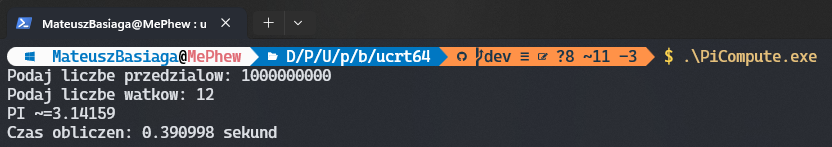
\includegraphics[width=\textwidth]{rys/program_example.png}
    \caption{Efekt działania programu}
    \label{rys:program_example}
  \end{center}
\end{figure}

Na rysunku \OznaczZdjecie{program_example} przedstawiono efekt działania programu dla liczby wątków równej 12 i liczby podziałów równej 1000000000.
Jak widać obliczenia zajęły jedynie około 0,39s.

\subsection{Testy wydajności programu}

\lstinputlisting[caption=Fragment kodu odpowiedzialny za uruchamianie trybu testu wydajności, label={lst:benchmark_main}, language=C++]{kod/benchmark_main.cpp}

Na listingu \OznaczKod{benchmark_main} przedstawiono fragment kodu odpowiedzialny za uruchamianie trybu testu wydajności w przypadku,
gdy program zostanie uruchomiony z parametrem \texttt{--benchmark}.

\newpage

\lstinputlisting[caption=Funkcja runBenchark odpowiedzialna za wykonanie pojedynczego testu wydajności, label={lst:run_benchmark}, language=C++]{kod/run_benchmark.cpp}

Funkcja \texttt{runBenchmark} (listing \OznaczKod{run_benchmark}), uruchamia algorytm dla danej liczby wątków oraz liczby podziałów, a następnie zapisuje wyniki do pliku \texttt{benchmark.csv}.
Na ich podstawie sporządzono arkusz programu Excel, pozwalający na szczegółową analizę wydajności programu.

\newpage

\begin{figure}[!htb]
  \begin{center}
    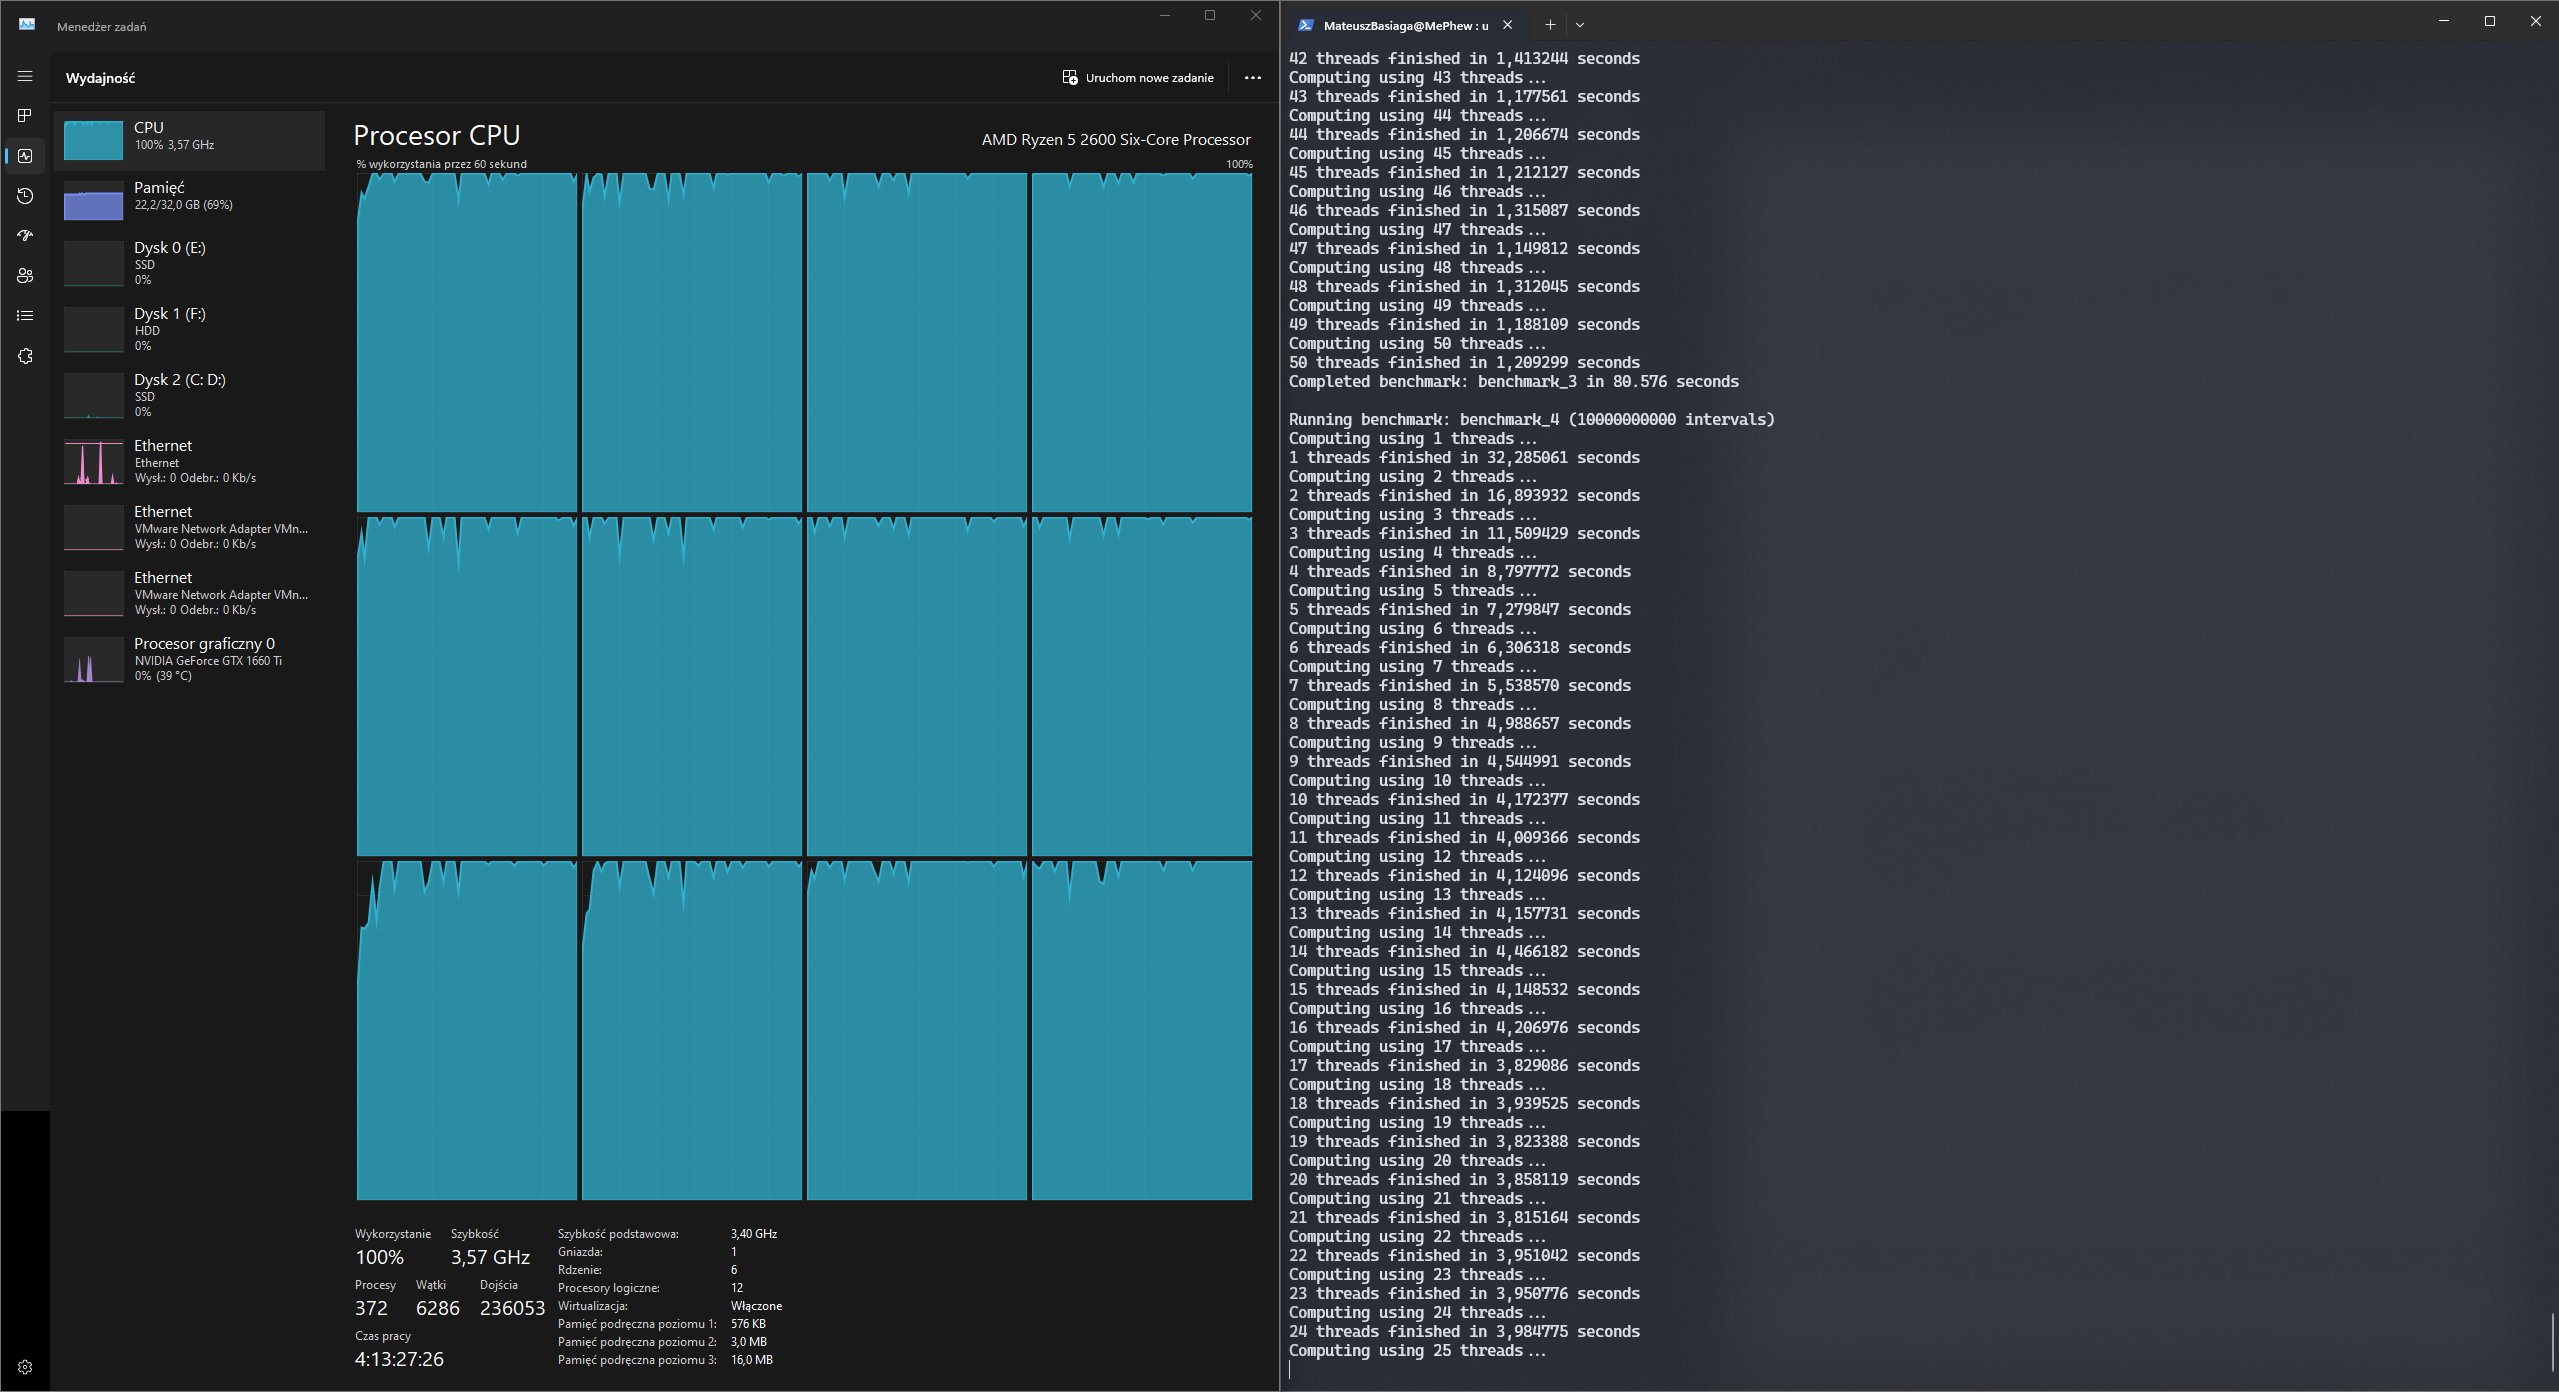
\includegraphics[width=\textwidth]{rys/computing_in_progress.png}
    \caption{Zużycie procesora podczas obliczeń}
    \label{rys:computing_in_progress}
  \end{center}
\end{figure}

Na rysunku \OznaczZdjecie{computing_in_progress} przedstawiono zużycie procesora podczas wykonywania testu wydajności.
Jak widać program jest bardzo zasobożerny.

\begin{figure}[!htb]
  \begin{center}
    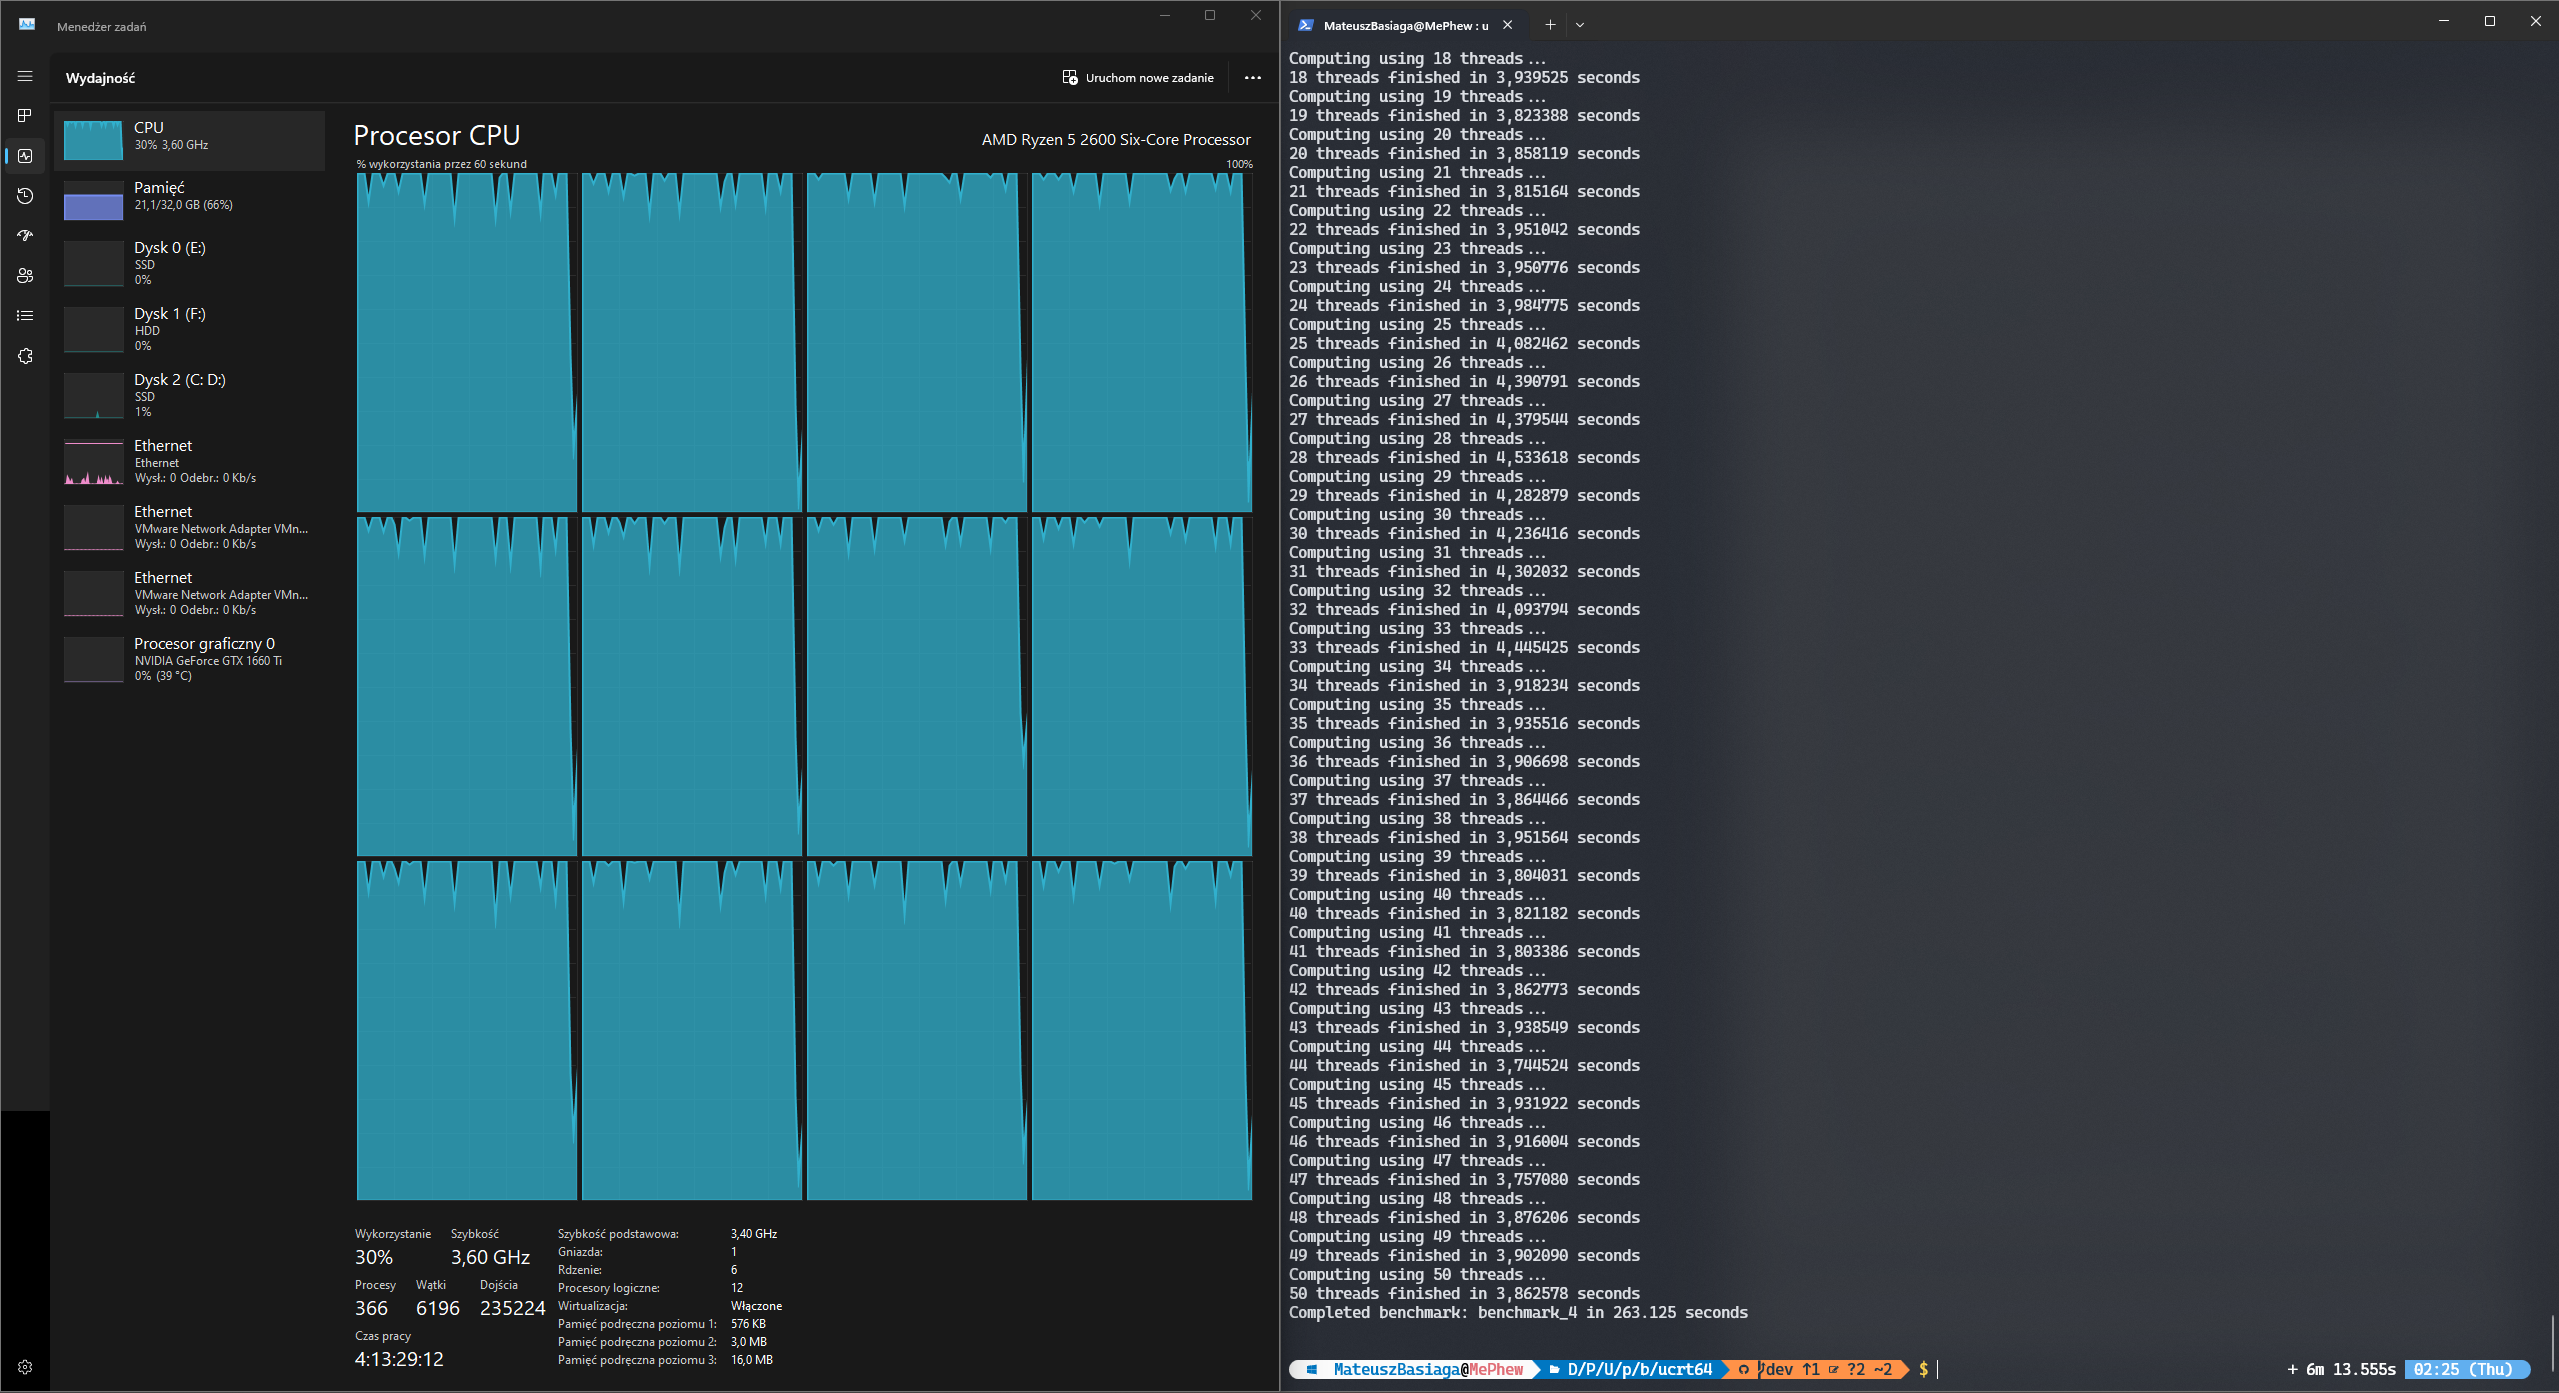
\includegraphics[width=\textwidth]{rys/computing_done.png}
    \caption{Zakończenie testu wydajności}
    \label{rys:computing_done}
  \end{center}
\end{figure}

Rysunek \OznaczZdjecie{computing_done} przedstawia zakończenie testu wydajności.
Jak widać przeprowadzenie całego testu zajęło niewiele ponad 263 sekundy (około 4 minuty).

\newpage

\begin{longtable}[c]{|c|l|l|l|l}
  \cline{1-4}
  \multicolumn{1}{|l|}{Wątki} & 10000000 & 1000000000 & 3000000000 & \\ \cline{1-4}
  \endfirsthead
  %
  \endhead
  %
  1                           & 1,01     & 9,898      & 30,1       & \\ \cline{1-4}
  2                           & 0,504    & 5,012      & 15,84      & \\ \cline{1-4}
  3                           & 0,344    & 3,423      & 11,123     & \\ \cline{1-4}
  4                           & 0,262    & 2,625      & 8,016      & \\ \cline{1-4}
  5                           & 0,213    & 2,114      & 6,475      & \\ \cline{1-4}
  6                           & 0,177    & 1,778      & 5,488      & \\ \cline{1-4}
  7                           & 0,154    & 1,539      & 4,884      & \\ \cline{1-4}
  8                           & 0,136    & 1,353      & 4,226      & \\ \cline{1-4}
  9                           & 0,121    & 1,233      & 3,696      & \\ \cline{1-4}
  10                          & 0,11     & 1,092      & 3,369      & \\ \cline{1-4}
  11                          & 0,104    & 1,003      & 3,071      & \\ \cline{1-4}
  12                          & 0,108    & 0,961      & 3,179      & \\ \cline{1-4}
  13                          & 0,12     & 1,074      & 3,196      & \\ \cline{1-4}
  14                          & 0,127    & 1,067      & 3,184      & \\ \cline{1-4}
  15                          & 0,144    & 1,036      & 3,12       & \\ \cline{1-4}
  16                          & 0,137    & 1,046      & 3,166      & \\ \cline{1-4}
  17                          & 0,129    & 1,037      & 2,959      & \\ \cline{1-4}
  18                          & 0,122    & 1,091      & 2,94       & \\ \cline{1-4}
  19                          & 0,117    & 1,005      & 3,133      & \\ \cline{1-4}
  20                          & 0,112    & 1,048      & 3,335      & \\ \cline{1-4}
  21                          & 0,111    & 1,061      & 3,214      & \\ \cline{1-4}
  22                          & 0,103    & 1,092      & 3,146      & \\ \cline{1-4}
  23                          & 0,124    & 1,046      & 3,378      & \\ \cline{1-4}
  24                          & 0,098    & 1,135      & 3,025      & \\ \cline{1-4}
  25                          & 0,125    & 1,113      & 3,292      & \\ \cline{1-4}
  26                          & 0,124    & 1,127      & 3,044      & \\ \cline{1-4}
  27                          & 0,121    & 1,029      & 3,253      & \\ \cline{1-4}
  28                          & 0,12     & 1,142      & 3,585      & \\ \cline{1-4}
  29                          & 0,113    & 1,016      & 3,115      & \\ \cline{1-4}
  30                          & 0,111    & 1,069      & 3,263      & \\ \cline{1-4}
  31                          & 0,108    & 1,043      & 3,017      & \\ \cline{1-4}
  32                          & 0,104    & 1,025      & 3,037      & \\ \cline{1-4}
  33                          & 0,103    & 1,035      & 3,235      & \\ \cline{1-4}
  34                          & 0,1      & 1,01       & 3,212      & \\ \cline{1-4}
  35                          & 0,102    & 0,998      & 3,133      & \\ \cline{1-4}
  36                          & 0,099    & 0,991      & 3,19       & \\ \cline{1-4}
  37                          & 0,119    & 0,98       & 3,186      & \\ \cline{1-4}
  38                          & 0,133    & 0,979      & 3,052      & \\ \cline{1-4}
  39                          & 0,113    & 0,987      & 3,154      & \\ \cline{1-4}
  40                          & 0,11     & 1,043      & 3,299      & \\ \cline{1-4}
  41                          & 0,108    & 0,98       & 3,14       & \\ \cline{1-4}
  42                          & 0,106    & 1,041      & 3,111      & \\ \cline{1-4}
  43                          & 0,103    & 1,011      & 3,119      & \\ \cline{1-4}
  44                          & 0,104    & 1,01       & 3,101      & \\ \cline{1-4}
  45                          & 0,101    & 1,004      & 2,981      & \\ \cline{1-4}
  46                          & 0,098    & 1,002      & 3,028      & \\ \cline{1-4}
  47                          & 0,099    & 1,026      & 3,08       & \\ \cline{1-4}
  48                          & 0,097    & 1,009      & 3,007      & \\ \cline{1-4}
  49                          & 0,112    & 0,985      & 2,976      & \\ \cline{1-4}
  50                          & 0,11     & 1,003      & 2,918      & \\ \hline
  \caption{Tabela zawierająca czas obliczeń dla poszczególnych wartości liczby podziałów w zależności od liczby wątków}
  \label{tab:computation_time_table}                                 \\
\end{longtable}

W tabeli \Oznacz{tab}{computation_time_table} przedstawiono tabelę z wynikami testów wydajności dla poszczególnych wartości liczby podziałów w zależności od ilości liczby wątków.

\newpage

\begin{figure}[!htb]
  \begin{center}
    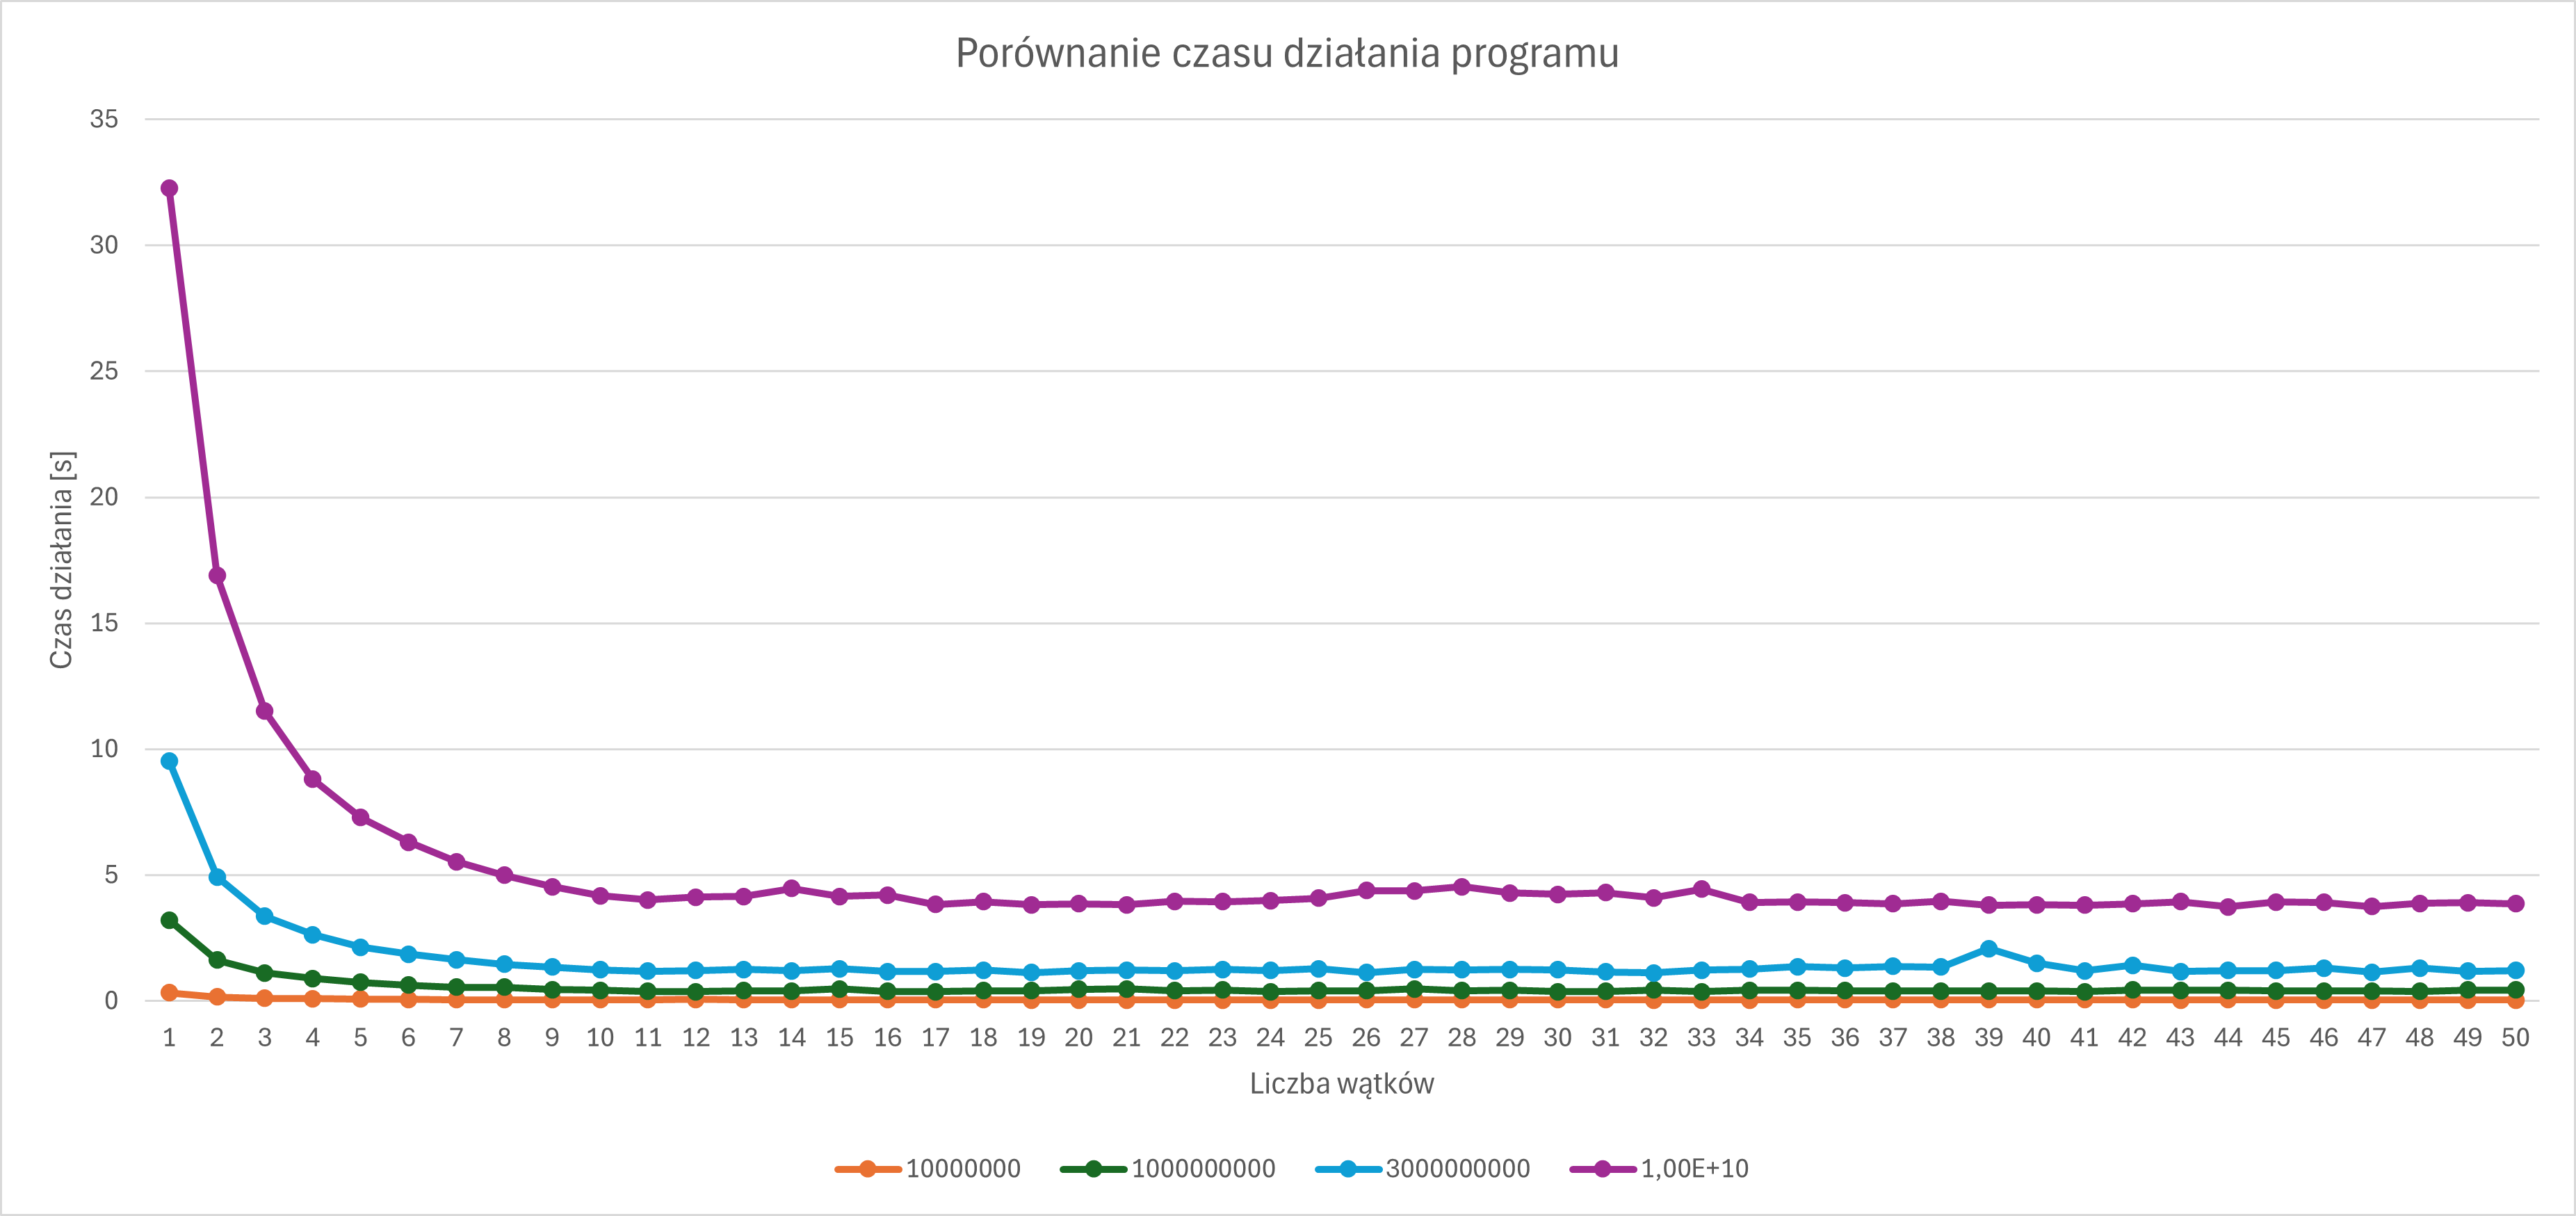
\includegraphics[width=\linewidth]{rys/computation_time_chart.png}
    \caption{Wykres czasu obliczeń dla poszczególnych wartości liczby podziałów w zależności od liczby wątków}
    \label{rys:computation_time_chart}
  \end{center}
\end{figure}

Na wykresie (rys. \OznaczZdjecie{computation_time_chart}) przedstawiono zależność czasu obliczeń od liczby wątków dla poszczególnych wartości liczby podziałów.
Różnice możemy zaobserwować przy większych liczbach podziałów, gdzie zwiększenie liczby wątków powoduje znaczne skrócenie czasu obliczeń.
Warto zauważyć, że po przekroczeniu liczby 12 wątków czas obliczeń nie ulega już znaczącej zmianie, co może wynikać z ograniczeń sprzętowych (ilość wątków procesora).
